%%%%%%%%%%%%%%%%%%%%%%%%%%%%%%%%%%%%%%%%%%%%%%%%%%%%%%%%%%%%%%%%%%%%%%%%%%%%%%%%
\documentclass[letterpaper, 10pt, conference]{ieeeconf}

\IEEEoverridecommandlockouts
\overrideIEEEmargins

% ── Packages ──────────────────────────────────────────────────────────────────
\usepackage{graphicx}
\usepackage{amsmath}
\usepackage{booktabs}
\usepackage{url}
\usepackage{cite}
\usepackage{tikz}
\usetikzlibrary{positioning, arrows.meta, shapes.geometric, calc, fit, backgrounds, decorations.pathreplacing}

% ieeeconf pre-defines a fake \NAT@parse to block natbib — clear it first.
\makeatletter
\let\NAT@parse\undefined
\makeatother
\usepackage[authoryear,round]{natbib}

% ── Title & Author ────────────────────────────────────────────────────────────
\title{\LARGE \bf
The EU Carbon Border Adjustment Mechanism and China's Strategic Response:
Carbon Pricing Realignment and Industrial Decarbonization
}

\author{Tang Qian \quad Sirawit Tangchitwatthanakon \quad Liu Xianghui \\
IPEN 6100: Global Environmental and Climate Policy \\
HKUST(GZ), Spring 2026
}
% ===== 页码设置 =====
\usepackage{fancyhdr}
\pagestyle{fancy}
\fancyhf{}
\fancyfoot[C]{\thepage}
\renewcommand{\headrulewidth}{0pt}
\renewcommand{\footrulewidth}{0pt}

\begin{document}

\maketitle
\thispagestyle{fancy} 



%%%%%%%%%%%%%%%%%%%%%%%%%%%%%%%%%%%%%%%%%%%%%%%%%%%%%%%%%%%%%%%%%%%%%%%%%%%%%%%%
\begin{abstract}
\normalfont
The European Union's Carbon Border Adjustment Mechanism (CBAM), entering its definitive phase in January 2026, operationalizes Nordhaus's climate club logic by linking market access to carbon pricing. This paper examines how CBAM reshapes China's carbon pricing architecture and sectoral decarbonization in steel and cement, the two sectors driving China's CBAM exposure. Using plant-level data from the Global Energy Monitor trackers (458 steel and 1{,}016 cement plants) and a liability model derived from Regulation EU 2023/956, we identify three transmission channels: a direct cost channel, a revenue retention incentive, and a signalling channel benchmarking CN-ETS ambition against EU ETS prices. At the prevailing price gap, BF-BOF steel exports face a net liability of EUR 140.7/t, versus EUR 6.7/t for EAF steel and EUR 42.1/t for cement---a 17.6:1 intensity ratio that maps directly onto competitiveness exposure. CN-ETS reforms announced since 2023---absolute caps by 2027, sectoral expansion, and gradual auctioning---correlate with, and are plausibly reinforced by, CBAM's fiscal logic, though domestic dual-carbon goals provide independent momentum and causal attribution lies beyond this study's scope. We contribute an empirically calibrated assessment of CBAM's first-year implementation and identify conditions under which trade-linked enforcement complements rather than substitutes for multilateral cooperation.

\medskip
\textbf{Keywords: CBAM; CN-ETS; carbon pricing convergence; industrial decarbonization}
\end{abstract}
%%%%%%%%%%%%%%%%%%%%%%%%%%%%%%%%%%%%%%%%%%%%%%%%%%%%%%%%%%%%%%%%%%%%%%%%%%%%%%%%
%  I. INTRODUCTION
%%%%%%%%%%%%%%%%%%%%%%%%%%%%%%%%%%%%%%%%%%%%%%%%%%%%%%%%%%%%%%%%%%%%%%%%%%%%%%%%
\section{Introduction}

\subsection{From Free-Riding to Trade-Linked Enforcement: Why CBAM Matters}

Global climate governance has long suffered from the tragedy of the atmospheric commons: mitigation benefits are universally shared, while abatement costs fall exclusively on individual jurisdictions \citep{Hardin1968}. This structural free-riding incentive has undermined every multilateral architecture, from the Kyoto Protocol's unenforceable targets to the Paris Agreement's voluntary NDCs. Nordhaus's \citeyearpar{Nordhaus2015} climate club proposal addresses this enforcement gap by proposing a coalition of high-ambition jurisdictions that adopt a common internal carbon price and impose uniform border tariffs on non-members, making free-riding costlier than abatement.

For nearly a decade, the climate club remained a theoretical construct. This changed with the CBAM, which entered its transitional phase in October 2023 and definitive phase in January 2026---the first instrument to operationalize trade-linked carbon enforcement at scale \citep{EURegulation2023}. Under Regulation EU 2023/956, importers of six carbon-intensive goods must surrender certificates priced at the weekly average EU ETS allowance price. Critically, verified carbon costs paid in the country of origin are deducted euro for euro from CBAM liability. This deduction clause is CBAM's strategic core: it transforms cross-border price differentials into a direct fiscal incentive for non-EU jurisdictions to strengthen domestic carbon pricing and retain revenue locally.

\subsection{CBAM's Particular Relevance for China}

As the EU's largest non-EU source of CBAM-liable imports, China represents the most consequential test case for the climate club model. Three factors define this relationship.

First, the carbon price gap is large and policy-actionable. In 2024--2025, EU ETS allowances traded at EUR 50--75/tCO\textsubscript{2} \citep{EURegulation2023}, while CN-ETS allowances cleared at EUR 10--13/tCO\textsubscript{2} \citep{MEE2023}. At an EU ETS price of EUR 80/tCO\textsubscript{2}, steel produced via the blast furnace--basic oxygen furnace (BF-BOF) route faces a net liability of EUR 140.7/t, compared to just EUR 6.7/t for electric arc furnace (EAF) steel---a 17.6:1 intensity ratio that directly maps emissions performance to competitiveness.

Second, China's industrial structure creates structural vulnerability. Its steel sector (458 plants, 1{,}005 Mtpa---million tonnes per annum---capacity, 54\% of global total) is 83.1\% BF-BOF based, compared to 44\% in the EU and 29\% globally \citep{WorldSteel2024}. Its cement industry (1{,}016 plants, 1{,}772 Mtpa capacity) has a clinker-to-cement ratio of 0.760, exceeding the global average of 0.73. The carbon-intensive technology mix that enabled China's industrialization is precisely what CBAM penalizes most heavily.

Third, CBAM's timeline aligns with a critical domestic reform window. Between 2023 and 2027, China's Ministry of Ecology and Environment announced three landmark CN-ETS reforms: transition to absolute emissions caps by 2027, expansion to steel and cement (2024), and gradual introduction of allowance auctioning \citep{MEE2021,MEE2023}. While China's ``dual carbon'' goals provide independent momentum, the temporal alignment with CBAM invites scrutiny of how external pressure interacts with domestic reform---an analytical task this paper takes up.

\subsection{Research Question, Scope, and Contribution}

This paper addresses the central question: \textit{How does CBAM reshape China's carbon pricing architecture and sectoral decarbonization pathways?} We decompose this into three sub-questions: (i) what channels transmit CBAM pressure to Chinese policymakers and industry; (ii) what is the magnitude of sectoral cost exposure under current and reformed CN-ETS scenarios; and (iii) what political-economy constraints bound feasible reform trajectories.

Our empirical analysis focuses on steel and cement during 2024--2027. Methodologically, we combine Global Energy Monitor plant-level data with a CBAM liability model derived directly from Regulation EU 2023/956.

This paper makes three contributions: (i) an empirically calibrated assessment of CBAM's first-year implementation, moving beyond pre-implementation modelling; (ii) a three-channel transmission framework linking CBAM design to CN-ETS reform; and (iii) a clarification of the climate club model's limits in non-OECD contexts.

The remainder of the paper proceeds as follows. Section II reviews the literature and identifies gaps. Section III describes data and methods. Section IV analyses CBAM design and transmission channels. Section V presents empirical results. Section VI examines industrial and policy responses. Section VII discusses implications. Section VIII concludes.

%%%%%%%%%%%%%%%%%%%%%%%%%%%%%%%%%%%%%%%%%%%%%%%%%%%%%%%%%%%%%%%%%%%%%%%%%%%%%%%%
%  II. LITERATURE REVIEW AND THEORETICAL FRAMEWORK
%%%%%%%%%%%%%%%%%%%%%%%%%%%%%%%%%%%%%%%%%%%%%%%%%%%%%%%%%%%%%%%%%%%%%%%%%%%%%%%%
\section{Literature Review and Theoretical Framework}
\label{sec:lit}

\subsection{Climate Clubs and the CBAM as a De Facto Club}
\label{sec:lit-clubs}

Nordhaus's \citeyearpar{Nordhaus2015} climate club model proposes that a coalition adopting a common internal carbon price and imposing \textit{uniform} penalty tariffs on non-members can sustain stable high-abatement coalitions. A growing literature examines whether the EU's CBAM operationalises this logic. Tagliapietra and Wolff \citeyearpar{Tagliapietra2021} and Szulecki et al.\ \citeyearpar{Szulecki2022} characterise CBAM as a ``de facto'' climate club, yet emphasise that its incentive structure diverges from Nordhaus's stylised model: rather than excluding non-members through uniform tariffs, CBAM's deduction clause creates a fiscal pull toward domestic carbon pricing. More fundamental critiques question whether the club mechanism captures the actual politics of climate cooperation. Falkner \citeyearpar{Falkner2016} and Falkner, Nasiritousi, and Reischl \citeyearpar{Falkner2022} argue that minilateral clubs face severe legitimacy and feasibility constraints, and that ``the most stringent climate club proposals are focused on overcoming the free-riding problem rather than addressing distributive conflict'' \citep{Falkner2022}. Aklin and Mildenberger \citeyearpar{Aklin2020} push this further, arguing that climate inaction reflects domestic distributive conflict, not international free-riding---governments adopt climate policies regardless of others' actions, suggesting external sanctions target the wrong binding constraint. Böhringer et al.\ \citeyearpar{Bohringer2022} and Mehling et al.\ \citeyearpar{Mehling2019} converge on a similar diagnosis from a design perspective: real-world border adjustments must accommodate vastly heterogeneous national circumstances, generating administrative and equivalence challenges that the homogenous-region Nordhaus framework abstracts away. This paper tests whether these heterogeneities undermine the climate club's self-enforcing logic in the Chinese context.

\subsection{Two-Level Games in Authoritarian Climate Governance}
\label{sec:lit-twolevel}

Putnam's \citeyearpar{Putnam1988} two-level game framework, in which negotiators simultaneously bargain at international and domestic tables constrained by overlapping ``win-sets,'' has become a standard lens for analysing climate diplomacy \citep{Bailer2012}. Its application to China requires substantial adaptation. The original framework presumes electoral ratification, whereas China's domestic ``Level II'' game is constructed through bureaucratic competition among ministries (MEE, NDRC, MIIT, MOFCOM), provincial fiscal interests, and state-owned enterprise lobbying \citep{Feng2021,Gilley2012}. Recent work by Chen and Lo \citeyearpar{ChenLo2025} on ``authoritarian environmentalism 2.0'' demonstrates that market-based instruments such as ETS reinforce hierarchical state control rather than constraining it---suggesting that international pressure interacts with Chinese policy through intra-state distributive bargaining rather than legislative veto. This reframing is consequential: external instruments such as CBAM enter Chinese policy debates not by changing aggregate national costs but by reshaping the relative bargaining position of pro-reform actors within the bureaucracy. We operationalise this logic by examining how CBAM's differential cost impacts across technologies and provinces alter the domestic win-set for CN-ETS reform.

\subsection{Carbon Pricing Convergence and ETS Diffusion}
\label{sec:lit-convergence}

The literature on ETS diffusion offers two contending expectations. The optimistic view---underlying linkage proposals from the EU--Switzerland model---anticipates convergence of design as jurisdictions emulate the EU template. The empirical record is more sobering: Wettestad and Gulbrandsen \citeyearpar{Wettestad2018} document that ETS diffusion has produced design \textit{divergence} more often than convergence, as local political-economy factors override technocratic emulation. China's case illustrates this divergence. Stoerk, Dudek, and Yang \citeyearpar{Stoerk2019} warned at CN-ETS launch that intensity-based caps with ex-post adjustment could undermine price signals---a critique now being addressed through the announced 2027 transition to absolute caps. Cui et al.\ \citeyearpar{Cui2021} provide firm-level evidence that even China's regional pilots reduced emissions by 16.7\% without significant output loss, suggesting that low headline prices need not imply policy ineffectiveness. Dai and Pollitt \citeyearpar{Dai2025}, drawing on extensive document and interview evidence, conclude that CN-ETS expansion is constrained primarily by MRV bottlenecks rather than political will, and that CBAM imposes an effective 2034 deadline for full CN-ETS maturity. Together, these studies suggest that CBAM does not produce convergence directly; it alters the political-economy calculus of jurisdictions whose pre-existing reform trajectories were already underway. This paper quantifies the magnitude of this ``accelerator effect'' by comparing CN-ETS reform timelines before and after CBAM's announcement.

\subsection{Empirical Evidence on CBAM's Post-Implementation Effects}
\label{sec:lit-empirical}

Until 2024, almost all CBAM impact assessments relied on pre-implementation modelling. Post-implementation empirical work remains sparse but is rapidly accumulating, with two methodologically distinct studies forming the baseline for our analysis. Li et al.\ \citeyearpar{Li2026}, using a global multi-regional input--output (GMRIO) framework, estimate that China's CBAM-induced export losses rise from EUR 0.78 billion under current scope to EUR 11.14 billion under full expansion, and find that CN-ETS can offset 30--60\% of these losses depending on price scenarios and CBAM coverage. Pan et al.\ \citeyearpar{Pan2025} couple GMRIO with the GCAM-China integrated assessment model at provincial resolution and report offset rates of 42\% (DICE model) to 49\% (ECE scenario) for iron and steel exports specifically, with over 65\% of provincial costs concentrated in Hebei, Jiangsu, Shanxi, Liaoning, and Zhejiang. The two estimates fall within overlapping ranges, but the divergence in headline figures reflects substantively different assumptions: Li covers all CBAM sectors with static GMRIO and price-scenario variation, while Pan focuses on ISAP with dynamic modelling that captures EAF technology penetration as a mitigation channel. The two studies are best read as complementary rather than competing, but neither traces the political-economy mechanism by which CBAM pressure becomes domestic CN-ETS reform.

Complementary evidence reinforces the picture: Magacho, Espagne, and Godin \citeyearpar{Magacho2024} establish the heterogeneity of CBAM exposure across EU trade partners; Wang et al.\ \citeyearpar{Wang2024} estimate that CBAM reduces Chinese steel exporters' profits by 58\% even as environmental benefits remain marginal at the sectoral level; Clausing et al.\ \citeyearpar{Clausing2025} document empirical instances of CBAM-induced policy diffusion, including China's March 2025 expansion of CN-ETS to CBAM-covered sectors. The divergence between Li et al.\ \citeyearpar{Li2026} and Pan et al.\ \citeyearpar{Pan2025} highlights a broader methodological limitation: static CGE models capture aggregate cost exposures but miss dynamic technology adjustment, while dynamic IAMs incorporate mitigation channels but rely on sector-average emission factors. This paper addresses both limitations by using plant-level data to model technology heterogeneity within a static liability framework calibrated to post-implementation policy parameters.

\subsection{Research Gaps and Analytical Framework}
\label{sec:lit-framework}
\begin{figure}[!h]
\centering
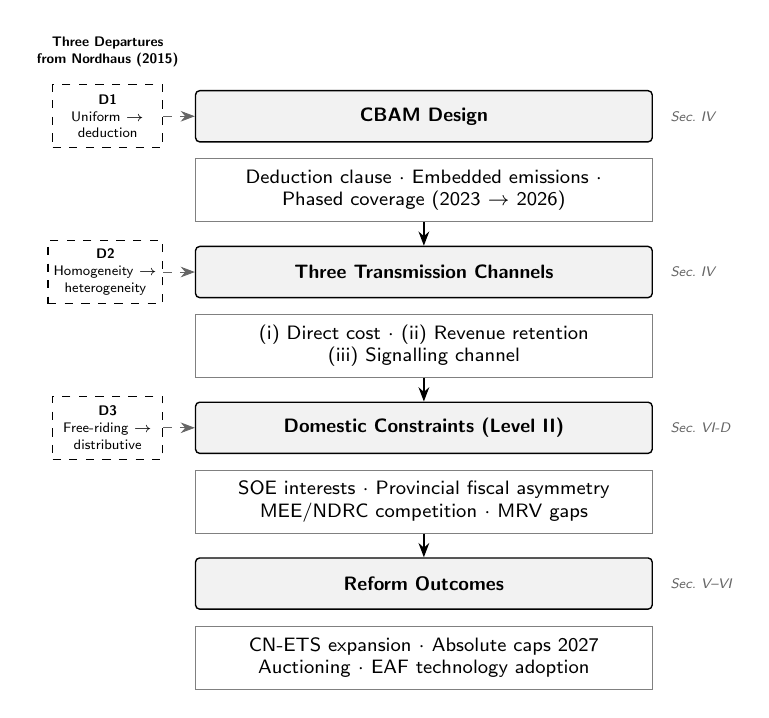
\begin{tikzpicture}[
    font=\sffamily\scriptsize,
    node distance=2mm,
    >={Stealth[length=1.8mm]},
    stage/.style={
        rectangle, rounded corners=1.5pt,
        draw=black, line width=0.5pt, fill=gray!10,
        minimum width=58mm, minimum height=6.5mm,
        align=center, font=\sffamily\bfseries\scriptsize
    },
    items/.style={
        rectangle, draw=black!50, line width=0.3pt, fill=white,
        minimum width=58mm, minimum height=8mm,
        align=center, font=\sffamily\scriptsize, inner sep=2.5pt
    },
    sect/.style={
        font=\sffamily\itshape\tiny, text=black!60
    },
    departure/.style={
        rectangle, draw=black, line width=0.4pt, dashed,
        fill=white, minimum width=14mm, minimum height=8mm,
        align=center, font=\sffamily\tiny, inner sep=2pt
    }
]

% ============ MAIN FLOW (vertical) ============
\node[stage] (s1) {CBAM Design};
\node[items, below=of s1] (i1)
    {Deduction clause $\cdot$ Embedded emissions $\cdot$ \\ Phased coverage (2023 $\to$ 2026)};

\node[stage, below=3mm of i1] (s2) {Three Transmission Channels};
\node[items, below=of s2] (i2)
    {(i) Direct cost $\cdot$ (ii) Revenue retention \\ (iii) Signalling channel};

\node[stage, below=3mm of i2] (s3) {Domestic Constraints (Level II)};
\node[items, below=of s3] (i3)
    {SOE interests $\cdot$ Provincial fiscal asymmetry \\ MEE/NDRC competition $\cdot$ MRV gaps};

\node[stage, below=3mm of i3] (s4) {Reform Outcomes};
\node[items, below=of s4] (i4)
    {CN-ETS expansion $\cdot$ Absolute caps 2027 \\ Auctioning $\cdot$ EAF technology adoption};

% ============ MAIN FLOW ARROWS ============
\draw[->, line width=0.7pt] (i1) -- (s2);
\draw[->, line width=0.7pt] (i2) -- (s3);
\draw[->, line width=0.7pt] (i3) -- (s4);

% ============ SECTION TAGS (right side) ============
\node[sect, right=1mm of s1] {Sec.~IV};
\node[sect, right=1mm of s2] {Sec.~IV};
\node[sect, right=1mm of s3] {Sec.~VI-D};
\node[sect, right=1mm of s4] {Sec.~V--VI};

% ============ THREE DEPARTURES (left side) ============
\node[departure, left=4mm of s1] (dep1) {\textbf{D1} \\ Uniform $\to$ \\ deduction};
\node[departure, left=4mm of s2] (dep2) {\textbf{D2} \\ Homogeneity $\to$ \\ heterogeneity};
\node[departure, left=4mm of s3] (dep3) {\textbf{D3} \\ Free-riding $\to$ \\ distributive};

% Dashed connectors
\draw[->, dashed, draw=black!60, line width=0.3pt] (dep1.east) -- (s1.west);
\draw[->, dashed, draw=black!60, line width=0.3pt] (dep2.east) -- (s2.west);
\draw[->, dashed, draw=black!60, line width=0.3pt] (dep3.east) -- (s3.west);

% Departures umbrella label
\node[font=\sffamily\bfseries\tiny, above=1mm of dep1.north,
      anchor=south, align=center]
    {Three Departures \\ from Nordhaus (2015)};

\end{tikzpicture}
\caption{Analytical framework. CBAM's design (Stage 1) generates three transmission channels (Stage 2) that interact with China's domestic political-economy constraints (Stage 3) to shape CN-ETS reform outcomes (Stage 4). Three departures from Nordhaus's stylised climate club (left, D1--D3) define the paper's theoretical contribution; Stage 3 constraints operationalise Putnam's Level II.}
\label{fig:framework}
\end{figure}
Synthesising the above literature, we identify three critical departures of CBAM from Nordhaus's stylised climate club model that have not been jointly theorised or empirically tested (summarised in Fig.~\ref{fig:framework}). \textit{First}, CBAM's deduction clause replaces Nordhaus's uniform tariff with a differentiated, emission-intensity-dependent liability that endogenises the choice of domestic carbon pricing---transforming the club mechanism from exclusionary tariff to gravitational fiscal pull. \textit{Second}, CBAM's non-member targets exhibit vast industrial-structure heterogeneity that Nordhaus's homogenous-region C-DICE framework cannot capture; China's BF-BOF dominance and provincial concentration of CBAM exposure \citep{Pan2025} generate response capacities and constraints fundamentally different from those of EU member states. \textit{Third}, the binding constraint on CN-ETS reform is not international free-riding but domestic distributive conflict among provincial governments, SOEs, and central reformers \citep{Aklin2020,Cui2021,Dai2025}---a constraint Nordhaus's external-enforcement logic does not address.

These departures motivate three core research gaps that this paper addresses:
\begin{enumerate}
    \item \textbf{Mechanism gap}: Existing CGE and IAM studies compute equilibrium offset outcomes without mapping the causal transmission mechanism from CBAM external pressure to specific CN-ETS reform measures.
    \item \textbf{Heterogeneity gap}: Sector-average emissions modelling obscures the plant-level technology heterogeneity that drives the BF-BOF--EAF cost differential central to China's adjustment pathway.
    \item \textbf{Context gap}: No study has systematically integrated domestic distributive conflict into an empirical assessment of CBAM's impact on non-OECD carbon pricing systems.
\end{enumerate}

To address these gaps, we develop a transmission-channel framework comprising the direct cost channel, the revenue retention incentive, and the signalling channel (Section IV), and apply it to plant-level data on China's steel and cement sectors (Sections V--VI). The framework operationalises Putnam's two-level logic in the authoritarian-bureaucratic context and integrates the distributive-conflict reading of climate politics into a tractable empirical assessment.


%  III. METHODOLOGY AND DATA
%%%%%%%%%%%%%%%%%%%%%%%%%%%%%%%%%%%%%%%%%%%%%%%%%%%%%%%%%%%%%%%%%%%%%%%%%%%%%%%%
\section{Methodology and Data}

\subsection{Data Sources}

Analysis draws on four primary datasets. Plant-level steel capacity and
technology data come from the GEM Iron \& Steel Tracker \citep{GEM_Steel2026},
comprising 458~operating plants with unit-level BOF/EAF technology
classification, provincial location, and production capacity. Cement
capacity data come from the GEM Cement and Concrete Tracker
\citep{GEM_Cement2025}, covering 1,016~operating plants with clinker
and cement capacity disaggregated by plant type (integrated
vs.\ grinding-only). Sectoral production benchmarks draw on
\citet{IEA2023} and \citet{WorldSteel2024}. Carbon pricing data for
the CN-ETS are sourced from MEE official publications
\citep{MEE2021, MEE2023}; EU ETS price ranges reflect 2024--2025
market data.

\subsection{Emission Factor Derivation}
\label{sec:emfactors}

Three sector-specific emission factors are applied throughout:

\textbf{BF-BOF steel: 2.10~tCO\textsubscript{2}/t} crude steel,
representing Scope~1 direct process emissions. WorldSteel (2024)
reports a global BF-BOF Scope~1+2 intensity of
2.34~tCO\textsubscript{2}/t \citep{WorldSteel2025}; Scope~1
constitutes the dominant component given near-exclusive reliance on
coking coal as blast furnace reductant, with purchased electricity
forming a minor share of total energy input.

\textbf{EAF steel: 0.10~tCO\textsubscript{2}/t} crude steel
(Scope~1, \textbf{CBAM-applicable only}). Under Regulation~EU
2023/956, Scope~2 (indirect) electricity emissions are
\textbf{excluded} from CBAM certificate liability for steel; only
Scope~1 direct process emissions apply. EAF Scope~1 of
0.10~tCO\textsubscript{2}/t reflects direct process emissions
\citep{WorldSteel2025}. For reference, WorldSteel (2025) reports
global scrap-EAF total intensity of 0.69~tCO\textsubscript{2}/t
including Scope~2 \citep{WorldSteel2025}. This total figure is
reported for technology comparison only and does \emph{not} affect
CBAM liability under Regulation~EU 2023/956. China's power generation
mix and associated grid emission factor are shown in
Fig.~\ref{fig:power_mix}.

\begin{figure}[htbp]
  \centering
  
\includegraphics[width=\columnwidth]{fig9_power_mix.png}
  \caption{China's power generation mix and associated grid emission
    factor (0.581~kgCO\textsubscript{2}/kWh) \citep{MEE2023}. Shown
    for reference; WorldSteel (2024) global scrap-EAF total intensity
    is 0.69~tCO\textsubscript{2}/t including Scope~2
    \citep{WorldSteel2025}. Scope~2 is excluded from CBAM liability
    for steel under Regulation~EU 2023/956 (Scope~1 only:
    0.10~tCO\textsubscript{2}/t).}
  \label{fig:power_mix}
\end{figure}

\textbf{Cement: 0.627~tCO\textsubscript{2}/t} finished cement,
derived from the GEM-observed clinker-to-cement ratio of 0.760
multiplied by the IPCC (2006) clinker emission factor of
0.825~tCO\textsubscript{2}/t clinker (calcination: 0.525; coal
combustion kiln heat: 0.300) \citep{IPCC2006}.

\subsection{CBAM Liability Model}
\label{sec:model}

Net CBAM liability per tonne of exported product $i$ is computed as:
%
\begin{equation}
  \text{CBAM Liability}_i =
    \max\!\bigl(0,\; EF_i \times (P_{\mathrm{EU}} - P_{\mathrm{CN}})\bigr)
  \label{eq:cbam_method}
\end{equation}
%
where $EF_i$ is embedded emissions intensity (tCO\textsubscript{2}/t),
$P_{\mathrm{EU}}$ is the prevailing EU ETS allowance price
(EUR/tCO\textsubscript{2}), and $P_{\mathrm{CN}}$ is the verified
CN-ETS carbon cost paid in the country of origin. Steel and cement
sectors entered CN-ETS coverage in 2024; $P_{\mathrm{CN}}$ therefore
reflects the prevailing CN-ETS allowance price for covered facilities,
currently EUR~10--13/tCO\textsubscript{2}. Sensitivity analysis spans
two EU ETS price scenarios (EUR~65 and EUR~80/tCO\textsubscript{2})
and five CN-ETS price states.

\subsection{Scope and Limitations}

Aggregate CBAM exposure estimates are bounded to current CBAM sectoral scope (HS Chapter~72
iron and steel; cement clinker); downstream embedded emissions in
manufactured goods are noted but not modelled. Provincial export
volumes are approximated from capacity shares rather than trade flow
data, introducing uncertainty in absolute cost estimates.

Causality is a further limitation: the correlation between CBAM
implementation and CN-ETS reform acceleration is consistent with the
analytical framework in Section~II.E, but formal causal identification
requires counterfactual evidence beyond the scope of this study.
Findings are interpreted as associations informed by theoretical
priors, not demonstrated causal effects. These parameters feed
directly into the liability model applied in Section~\ref{sec:results}.

%%%%%%%%%%%%%%%%%%%%%%%%%%%%%%%%%%%%%%%%%%%%%%%%%%%%%%%%%%%%%%%%%%%%%%%%%%%%%%%%
%  IV. CBAM DESIGN AND TRANSMISSION MECHANISMS
%  (Policy design + transmission logic only — no empirical exposure data)
%%%%%%%%%%%%%%%%%%%%%%%%%%%%%%%%%%%%%%%%%%%%%%%%%%%%%%%%%%%%%%%%%%%%%%%%%%%%%%%%
\section{CBAM Design and Transmission Mechanisms}

\subsection{Policy Design and Transmission Logic}
\label{sec:channels}

CBAM (Regulation~EU 2023/956) entered its definitive phase on
1~January~2026, following a transitional reporting-only phase from
1~October~2023 through 31~December~2025 \citep{EURegulation2023}. EU
importers of products listed in Annex~I---iron and steel,
cement, fertilisers, electricity, and hydrogen---must now register as
authorised CBAM declarants, surrender CBAM certificates by 31~May
each year against the preceding calendar year's verified embedded
emissions, and reconcile any outstanding liability with EU customs.
Certificate prices track the weekly auction-clearing price of EU~ETS
allowances, ensuring price equivalence between domestic compliance
and border-adjusted imports.

Embedded emissions are defined as Scope~1 direct emissions for steel
and hydrogen, with Scope~2 indirect electricity-related
emissions added for cement and fertilisers. Where verified
installation-level data are unavailable, default values published by
the European Commission apply; these are typically benchmarked at the
worst-decile producers globally, generating a strong incentive for
facility-level monitoring, reporting, and verification (MRV).

CBAM's strategic significance for China rests on Article~9 of the
Regulation, which permits the deduction of carbon costs already paid
in the country of origin from CBAM liability on a euro-for-euro basis,
provided those costs are verifiable and meet equivalence criteria
specified in implementing regulations. This deduction clause is the
fulcrum of the mechanism's interaction with Chinese carbon policy:
each yuan of effective CN-ETS compliance cost converts what would
otherwise be a transfer to the EU budget into revenue retained
domestically. The parallel free-allocation phase-out under EU~ETS
Annex~I---running 2026--2034 in linear annual decrements---calibrates
CBAM coverage to internal carbon-cost equalisation rather than
additional protection, a design feature critical to WTO defensibility.

Three transmission channels follow from this architecture and are
tested empirically in Sections~\ref{sec:results} and~\ref{sec:response}:

\begin{itemize}
  \item The \textbf{direct cost channel}: CBAM raises the landed
        cost of Chinese exports in proportion to embedded emissions
        intensity, with the per-tonne liability given by
        Eq.~\ref{eq:cbam_method}. The competitiveness implication
        scales with the Chinese carbon-intensity disadvantage relative
        to EU producers operating under stringent ETS prices.
  \item The \textbf{revenue retention incentive}: the Article~9
        deduction transforms domestic carbon pricing from a pure
        compliance cost into a fiscal-substitution instrument. Each
        marginal increase in $P_{\mathrm{CN}}$ shifts an equivalent
        quantum of revenue from EU coffers to Chinese ones, bounded
        above by $P_{\mathrm{EU}}$. This converts a passive
        trade-policy exposure into an active strategic incentive for
        CN-ETS reform.
  \item The \textbf{signalling channel}: the publicly observable
        $P_{\mathrm{EU}}$ functions as an external benchmark for
        CN-ETS ambition. Even where direct deduction logic is
        incomplete (e.g., during sectoral phase-in delays), the price
        gap is read by domestic policy actors---MEE, NDRC, sectoral
        associations---as an indicator of how far the reform agenda
        must travel.
\end{itemize}

A fourth, procedural channel emerges indirectly from MRV requirements:
CBAM's documentation standards effectively impose ISO~14064-aligned
carbon accounting on Chinese exporters as a precondition for accessing
facility-specific (rather than punitive default) emission factors.
From the firm's perspective this is sunk compliance cost; from the
system's perspective it is a public-good investment in carbon-market
infrastructure that complements CN-ETS expansion---an interaction
\citet{Dai2025} document as a binding bottleneck on CN-ETS maturity.

\subsection{Comparative Architecture: EU ETS and CN-ETS}
\label{sec:ets-comparison}

CBAM's revenue-retention logic operates entirely through the price gap
between the two emissions trading systems on either side of the
Article~9 deduction. Understanding the structural drivers of that gap
requires direct comparison of EU~ETS and CN-ETS architectures,
summarised in Table~\ref{tab:ets-comparison}.

\begin{table*}[!t]
\caption{Structural Comparison of EU~ETS and CN-ETS (2024--2025)}
\label{tab:ets-comparison}
\centering
\renewcommand{\arraystretch}{1.20}
\footnotesize
\begin{tabular}{p{2.6cm}|p{6.4cm}|p{6.4cm}}
\toprule
\textbf{Dimension} & \textbf{EU~ETS} & \textbf{CN-ETS} \\
\midrule
Year established
  & 2005 (Phase~I); Phase~IV running 2021--2030
  & 2021 (national); regional pilots from 2013 \\
\midrule
Sectoral coverage
  & Power, energy-intensive industry, intra-EEA aviation, maritime (from 2024)
  & Power generation; steel and cement (from 2024) \\
\midrule
Cap design
  & Absolute, declining; Linear Reduction Factor 4.3\% (2024--27), 4.4\% (2028--30)
  & Intensity-based; transition to absolute cap announced for 2027 \\
\midrule
Allocation method
  & Hybrid: auctioning ($\sim$57\%); free benchmark-based allocation declining via cross-sectoral correction factor
  & Free allocation against intensity benchmarks; auctioning pilots in select provinces \\
\midrule
Price (2024--25)
  & EUR~50--80 / tCO\textsubscript{2}
  & EUR~10--13 / tCO\textsubscript{2} (CNY~80--105) \\
\midrule
MRV regime
  & Accredited third-party verifiers under ISO~14065; central registry
  & Sectoral verifiers under MEE supervision; provincial registries integrating into national \\
\midrule
Compliance penalty
  & EUR~100/tCO\textsubscript{2} + missed-allowance surrender + name disclosure
  & Administrative penalty typically 5--10$\times$ market price; reform pending \\
\midrule
Linkage capability
  & Linked with Swiss ETS since 2020
  & No active linkage; bilateral cooperation under exploration \\
\midrule
Revenue use
  & Member states (climate purposes $\geq$50\%); Innovation Fund; Modernisation Fund
  & MEE; sectoral allocations; reform direction toward general fiscal absorption \\
\midrule
Offsets
  & Limited international credits, no longer accepted post-Phase~III
  & CCER (China Certified Emission Reductions) reactivated 2024, capped \\
\bottomrule
\end{tabular}
\end{table*}

The EUR~40--65 / tCO\textsubscript{2} price gap is structurally
generated by three differences. \textit{First}, EU~ETS imposes an
absolute cap whose annual contraction is mechanically priced into the
forward curve, whereas CN-ETS intensity benchmarking allows allowance
volumes to expand with output, dampening upward price pressure
\citep{Stoerk2019,Dai2025}. \textit{Second}, EU allocation has been
steadily migrating from free to auctioned, raising effective
compliance costs in line with the cap, while Chinese steel and cement
entered CN-ETS in 2024 with generous free allocation to ease the
transition. \textit{Third}, EU~ETS coverage spans the bulk of
stationary-combustion and industrial emissions, while CN-ETS covered
only the power sector through 2023 and remains in mid-expansion.

These structural features are the binding constraint on convergence.
Within the two-level games framework adopted in
Section~\ref{sec:lit-twolevel}, they define the upper limit of how
rapidly CN-ETS can be tightened without compromising sectoral
employment and energy-security imperatives \citep{Nahm2021}. CBAM
enters this domestic equilibrium as an external incentive that shifts
the cost--benefit calculation of reform---not by mandating convergence
but by attaching a measurable fiscal-leakage cost to non-convergence.

\subsection{Sectoral Coverage Logic and Expansion Trajectory}
\label{sec:coverage}

The sectors selected for CBAM Annex~I coverage---cement, iron and
steel, fertilisers, electricity, and hydrogen---share three
features that define the mechanism's analytical logic. \textit{First},
each is highly carbon-intensive, with embedded emissions in the range
of 0.6--2.1~tCO\textsubscript{2} per tonne of finished product.
\textit{Second}, each has documented exposure to carbon leakage under
the EU~ETS prior to CBAM, evidenced by free-allocation eligibility and
trade-intensity metrics maintained by the European Commission.
\textit{Third}, each is technologically mature enough to permit
reasonably standardised emission-factor methodologies, securing
administrative feasibility within a customs-based system.

Hydrogen and electricity are forward-looking inclusions. Hydrogen
exposure is currently small but anticipated to grow as the EU's
Renewable Energy Directive recast (RED~III) drives demand for
low-carbon hydrogen imports; electricity inclusion addresses
cross-border grid leakage from non-EU jurisdictions adjacent to EU
member states (Western Balkans, Türkiye), and is of limited direct
relevance for China.

The phase-in trajectory is designed for parallelism with EU~ETS
free-allocation reduction. Free allowances for CBAM-covered EU sectors
decline from 100\% in 2025 to 0\% in 2034 in linear annual decrements;
CBAM certificate obligations rise correspondingly, ensuring that
European producers always face the full carbon cost of their emissions
and that Chinese exporters face an equivalent cost on the residual
gap not covered by CN-ETS payments. This calibration is critical both
to WTO defensibility and to the mechanism's framing as equalisation
rather than protection.

Two expansion vectors are particularly consequential for China. The
first is the 2025--26 mandated review of CBAM scope, widely expected
to recommend extension to organic chemicals, polymers, and selected
downstream manufactured goods (refined steel products,
cement-based construction materials).
\citet{Li2026} project that this expansion would lift China's
aggregate CBAM exposure from EUR~0.78~billion under current pilot
scope to EUR~11.14~billion under full coverage---a 14$\times$ increase
reflecting both higher product volumes and the deeper integration of
CBAM-regulated inputs into Chinese manufacturing exports. The second
vector is the expansion of indirect (Scope~2) emissions coverage.
Currently included only for cement and fertilisers, the inclusion of
Scope~2 for steel would substantially raise the
per-tonne liability of Chinese producers reliant on coal-dominant
grids; the elasticity of this exposure to provincial grid factors is
quantified in Section~\ref{sec:robustness}.

\subsection{Strategic Foresight: CBAM as a Precedent for Global Border Carbon Adjustments}
\label{sec:foresight}

CBAM is no longer a single-jurisdiction risk for Chinese exporters.
The United Kingdom has confirmed that its own CBAM will enter force on
1~January~2027, covering cement, fertilisers, hydrogen, and
iron and steel under primary legislation enacted in the Finance
Act~2026, with secondary legislation under technical consultation
through mid-2026 \citep{HMRC2026}. The UK design parallels the EU
regime but excludes electricity and operates with a single global
default value per CN code in its first year, simplifying
administration at the cost of country-of-origin differentiation. The
UK and EU concluded an agreement in principle in May~2025 to link
their respective ETS systems and explore mutual CBAM exemption,
which would consolidate a transatlantic European carbon-pricing zone
with implications for Chinese MRV-equivalence negotiations.

In the United States, the bipartisan Foreign Pollution Fee Act of
2025 (S.~1325) was reintroduced in April~2025 by Senators Cassidy and
Graham, proposing tiered tariffs on imports of iron, steel,
cement, glass, fertilisers, hydrogen, and selected critical-mineral
and battery inputs \citep{Cassidy2025}. Unlike the EU and UK
mechanisms, the US proposal does not impose a domestic carbon price
and does not formally credit foreign carbon costs; it computes
pollution-intensity differentials relative to US production and
applies ad valorem tariffs accordingly. This design departs from the
price-equivalence logic of EU~CBAM and would, if enacted, expose
Chinese producers to a parallel charge with no offset pathway through
CN-ETS payments. Whether the bill advances is uncertain---prior
versions stalled in 2023--24---but its bipartisan support and explicit
geopolitical framing against China give it material policy weight
\citep{CSIS2024}. The accompanying PROVE~IT Act, which would direct
the U.S. Department of Energy to study comparative carbon intensities,
advanced from committee in the 118th Congress and provides the data
infrastructure on which any subsequent border-adjustment regime would
rely.

Canada's federal climate plan under the Carney government has
indicated active consideration of a CBAM as part of its 2030
industrial-policy package, and Australia conducted public
consultations on a Carbon Leakage Review concluding in 2024. While
neither jurisdiction has confirmed implementation, the cumulative
direction of policy diffusion is unambiguous: the EU's first-mover
act has shifted the equilibrium of acceptable trade--climate policy,
and China should plan for cumulative exposure to multiple, partially
overlapping border-adjustment regimes by 2028--30 rather than for the
EU mechanism in isolation.

This diffusion has two strategic implications. First, the marginal
value of strengthening CN-ETS rises with each additional jurisdiction
adopting deduction-based CBAMs, since the same domestic carbon cost
is increasingly offsettable across multiple borders. Second, the
heterogeneity of mechanism designs---deduction-based (EU, UK) versus
differential-based (US)---means that no single CN-ETS reform pathway
optimises against all of them simultaneously; harmonisation pressures
in MRV standards and verifier accreditation will likely intensify,
whether through bilateral mutual-recognition agreements or
multilateral fora such as the OECD Inclusive Forum on Carbon
Mitigation Approaches (IFCMA).

%%%%%%%%%%%%%%%%%%%%%%%%%%%%%%%%%%%%%%%%%%%%%%%%%%%%%%%%%%%%%%%%%%%%%%%%%%%%%%%%
%  V. EMPIRICAL RESULTS
%  A. Sectoral Exposure → B. Cost Quantification → C. Price Convergence
%%%%%%%%%%%%%%%%%%%%%%%%%%%%%%%%%%%%%%%%%%%%%%%%%%%%%%%%%%%%%%%%%%%%%%%%%%%%%%%%
\section{Empirical Results}
\label{sec:results}

\subsection{Sectoral Exposure: China's CBAM Vulnerability}
\label{sec:exposure}

China constitutes the single largest non-EU source country for
CBAM-liable exports, with exposure concentrated in steel and cement.

\textbf{Steel.} China's GEM-tracked steel industry comprises
458~plants with 1,005~Mtpa of operating crude steel production
capacity---approximately 54\% of global crude steel production
\citep{WorldSteel2024}. Of this capacity, 835.7~Mtpa (83.1\%) is
attributable to BF-BOF operations and 169.5~Mtpa (16.9\%) to EAF.
China's EAF share relative to global peers is shown in
Fig.~\ref{fig:eaf_share}. China's weighted-average CBAM-applicable emissions intensity (Scope~1)
across its current production mix is $0.831 \times 2.10 + 0.169
\times 0.10 = 1.76$~tCO\textsubscript{2}/t, vs.\
0.10~tCO\textsubscript{2}/t for a pure EAF producer---a 17.6:1 ratio
that translates directly into the core CBAM competitiveness liability.

\begin{figure}[htbp]
  \centering
  
\includegraphics[width=\columnwidth]{figA_eaf_share_by_country.png}
  \caption{EAF share of crude steel production capacity (\%) by
    country. China's 16.9\% compares with $\approx$29\% globally and
    $\approx$44\% in the EU, and $>$70\% in the United States
    \citep{WorldSteel2024}. Data: GEM Iron \& Steel Tracker,
    March 2026 \citep{GEM_Steel2026}.}
  \label{fig:eaf_share}
\end{figure}

\citet{Li2026} estimate aggregate CBAM-induced export losses rising from
EUR~0.78~billion under the current pilot sectors to EUR~11.14~billion with
full CBAM expansion across all covered products.
\citet{Pan2025} project CBAM costs of EUR~1,157~million by 2034 for
China's iron, steel, and aluminium exports to the EU, with over 65\%
of the burden falling on Hebei, Jiangsu, Shanxi, Liaoning, and
Zhejiang. Provincial BF-BOF capacity distribution underlying this
geographic concentration is shown in Fig.~\ref{fig:provinces}.
Actual exposure depends on export orientation; inland capacity
serving domestic markets may face lower realized CBAM costs than
coastal export-oriented capacity of equivalent scale.

\begin{figure}[htbp]
  \centering
  
\includegraphics[width=\columnwidth]{fig2_steel_provinces.png}
  \caption{Operating BOF and EAF capacity (Mtpa) by province, China.
    Hebei (199.7~Mtpa BOF), Jiangsu (86.8), Liaoning (69.5), Shanxi
    (53.2), and Shandong (52.0) collectively account for 55.2\% of
    national BOF capacity. Data: GEM Iron \& Steel Tracker,
    March 2026 \citep{GEM_Steel2026}.}
  \label{fig:provinces}
\end{figure}

\textbf{Cement.} China accounts for approximately 50--51\% of global
cement output \citep{GCCA2024}. GEM identifies 1,016~operating plants
with 1,772~Mtpa cement capacity and 1,346~Mtpa clinker capacity. At
the IPCC (2006) clinker emission factor of
0.825~tCO\textsubscript{2}/t clinker \citep{IPCC2006}, Chinese
integrated plants emit approximately 0.627~tCO\textsubscript{2}/t of
finished cement. Direct CBAM exposure from cement exports to the EU
is currently limited but would enlarge substantially under any
downstream construction materials expansion. The absence of large
direct flows does not eliminate exposure: cement is embedded in
higher-value construction products (precast elements, ready-mix
concrete) whose Scope~3 emissions could fall within future CBAM
reviews, and China's cement-export profile is heavily oriented toward
emerging-market construction markets where any climate-club expansion
would have second-order trade implications.

\textbf{Aluminium.} Aluminium is excluded from quantitative analysis
in this paper due to the absence of GEM unit-level smelting data for
China; the qualitative profile, however, merits sectoral treatment
because the structural features differ materially from those of steel
and cement.

China produces approximately 57\% of global primary aluminium \citep{Lou2025}, with
two structurally distinct production profiles defined by power-source
mix. Coal-dominant smelting concentrated in Xinjiang, Inner Mongolia,
and Shandong typically embodies more than 20~tCO\textsubscript{2}/t~Al \citep{Chatterjee2026},
dominated by Scope~2 indirect emissions from coal-fired captive power.
Hydropower-based smelting in Yunnan and Sichuan typically embodies
3--4~tCO\textsubscript{2}/t~Al, an order of magnitude lower. The
national weighted average lies in the 15--17~tCO\textsubscript{2}/t~Al
range \citep{Chatterjee2026}, roughly 2$\times$ the EU average
($\approx$6.5~tCO\textsubscript{2}/t~Al under current grid mix) \citep{EurAl2025}.

Direct CBAM exposure for primary aluminium is moderate---Chinese
primary aluminium exports to the EU are constrained by EU
anti-dumping measures and capacity-utilisation
constraints---but exposure through semi-fabricated products
(extrusions, plates, foil) is substantial. The CBAM Annex~I currently
covers selected primary and semi-fabricated aluminium products; the
2026 review is expected to consider expansion to downstream aluminium
goods (automotive parts, packaging), which would dramatically
increase exposure.

The strategic implication is that aluminium's CBAM cost is highly
dispatchable across provinces: contracting EU-bound smelting volumes
to hydropower-rich provinces would lower per-tonne liability by
EUR~10--15/t per tCO\textsubscript{2} of intensity reduction at
$P_{\mathrm{EU}}=$ EUR~65/tCO\textsubscript{2}, a far larger
differential than the steel BF-BOF/EAF gap. Aluminium thus represents
the sector with the largest potential for short-term CBAM-cost
arbitrage through within-China relocation, distinct from the deeper
technology-replacement requirements in steel.

\subsection{CBAM Cost Quantification}
\label{sec:sensitivity}

Applying Eq.~\ref{eq:cbam_method} with emission factors from
Section~\ref{sec:emfactors}, and with steel and cement carrying
$P_{\mathrm{CN}} \approx$ EUR~10--13/tCO\textsubscript{2} following
their 2024 CN-ETS inclusion, net CBAM liability per tonne is given in
Table~\ref{tab:cbam_liability} and visualized in
Fig.~\ref{fig:cbam_heatmap}.

\begin{figure}[htbp]
  \centering
  
\includegraphics[width=\columnwidth]{fig4_cbam_heatmap.png}
  \caption{Heatmap of net CBAM liability (EUR/t) across EU ETS price
    scenarios and CN-ETS coverage levels for BF-BOF steel, EAF steel,
    and cement. Derived from Table~\ref{tab:cbam_liability}.}
  \label{fig:cbam_heatmap}
\end{figure}

\begin{table*}[t]
\caption{Net CBAM Liability per Tonne of Product by CN-ETS Coverage
  and Price Scenario (EUR/t)}
\label{tab:cbam_liability}
\centering
\small
\begin{tabular}{lrrrrrr}
\toprule
 & \multicolumn{3}{c}{\textbf{EU ETS = EUR 65/tCO\textsubscript{2}}}
 & \multicolumn{3}{c}{\textbf{EU ETS = EUR 80/tCO\textsubscript{2}}} \\
\cmidrule(lr){2-4}\cmidrule(lr){5-7}
\textbf{CN-ETS Scenario}
  & \textbf{BF-BOF} & \textbf{EAF} & \textbf{Cement}
  & \textbf{BF-BOF} & \textbf{EAF} & \textbf{Cement} \\
\midrule
Not covered (pre-2024 baseline)                          & 136.5 &  6.5 & 40.8 & 168.0 &  8.0 & 50.2 \\
Covered, EUR~13/tCO\textsubscript{2} (\textit{current}) & 109.2 &  5.2 & 32.6 & 140.7 &  6.7 & 42.1 \\
Covered, EUR~40/tCO\textsubscript{2}                    &  52.5 &  2.5 & 15.7 &  84.0 &  4.0 & 25.1 \\
Covered, EUR~60/tCO\textsubscript{2}                    &  10.5 &  0.5 &  3.1 &  42.0 &  2.0 & 12.5 \\
Full parity (EU ETS level)                               &   0.0 &  0.0 &  0.0 &   0.0 &  0.0 &  0.0 \\
\bottomrule
\end{tabular}
\\[4pt]
\begin{minipage}{0.95\linewidth}
\footnotesize\textit{Note:} Emission factors: BF-BOF
2.10~tCO\textsubscript{2}/t Scope~1 (WorldSteel 2025 global
Scope~1+2: 2.34~tCO\textsubscript{2}/t; \citealt{WorldSteel2025});
EAF \textbf{0.10~tCO\textsubscript{2}/t Scope~1 only}
(CBAM-applicable; Scope~2 excluded per Regulation~EU 2023/956;
global scrap-EAF total 0.69~tCO\textsubscript{2}/t including Scope~2;
\citealt{WorldSteel2025}); Cement
0.627~tCO\textsubscript{2}/t (GEM clinker ratio
0.760~$\times$~IPCC 0.825~tCO\textsubscript{2}/t clinker;
\citealt{IPCC2006}). ``Pre-2024 baseline'' row assumes
$P_{\mathrm{CN}}=0$; ``current'' row reflects CN-ETS entry of steel
and cement in 2024 at EUR~13/tCO\textsubscript{2}.
Figures rounded to one decimal place.
\end{minipage}
\end{table*}

\textbf{Aggregate fiscal exposure.} Aggregate CBAM cost depends
jointly on per-tonne liability, EU-bound export volumes by sector,
and the EU~ETS price scenario. Under the current pilot scope and
current carbon-price gap, \citet{Li2026} and \citet{Pan2025} jointly
bound the annual fiscal exposure at EUR~0.78--1.16~billion, with the
latter rising to EUR~1.16~billion by 2034 in their projection. Under
the post-2026-review scope expansion, \citet{Li2026} project a ceiling
of EUR~11.14~billion. We treat these figures as outer bounds rather
than central estimates, given heterogeneity in underlying methodology:
\citet{Pan2025} construct estimates from province-level capacity data
within a dynamic IAM, while \citet{Li2026} employ static GMRIO that
captures sectoral input--output linkages including indirect downstream
exposure absent from the former.

\textbf{Provincial burden distribution.} The provincial allocation of
this fiscal exposure is highly skewed. \citet{Pan2025} attribute over
65\% of projected CBAM costs to five provinces---Hebei, Jiangsu,
Shanxi, Liaoning, and Zhejiang---broadly tracking BF-BOF capacity
distribution (Fig.~\ref{fig:provinces}). Hebei alone bears an
estimated 23\% of the national burden under their methodology. This
concentration creates an asymmetric political economy of reform: a
small set of provincial governments would bear most of the visible
cost, but national-level fiscal benefits from CN-ETS revenue retention
accrue centrally, generating intergovernmental coordination challenges
that the analytical framework in
Section~\ref{sec:lit-twolevel} treats as an extension of Putnam's
two-level logic to subnational federal-style bargaining.

\textbf{Sensitivity to emission factors.} The base case uses point
estimates for emission factors (BF-BOF 2.10, EAF Scope~1 only 0.10,
cement 0.627~tCO\textsubscript{2}/t). Plausible ranges around these,
drawn from \citet{IEA2023}, GEM unit-level data, and \citet{IPCC2006},
are: BF-BOF 1.95--2.30, EAF Scope~1 0.08--0.12, cement
0.58--0.68~tCO\textsubscript{2}/t. Because Eq.~\ref{eq:cbam_method}
is linear in $EF_i$, the per-tonne liability scales proportionally
with the emission factor: a $\pm$10\% deviation in BF-BOF intensity
translates into a $\pm$10\% deviation in BF-BOF liability, and
similarly for cement and EAF. The qualitative ranking
BF-BOF~$\gg$~cement~$>$~EAF (Scope~1) is preserved across the entire
plausible range, since the gaps between sectoral intensities exceed
the within-sector uncertainty by an order of magnitude. The
provincial grid-factor question, which matters for any future Scope~2
extension, is treated separately in Section~\ref{sec:robustness}.

\subsection{Carbon Price Gap and Convergence Scenarios}

As of 2024--2025, the EU ETS price has traded at
EUR~50--75/tCO\textsubscript{2} vs.\ EUR~10--13/tCO\textsubscript{2}
for CN-ETS. Three convergence scenarios toward full CBAM offset are
illustrated in Fig.~\ref{fig:price_convergence}.
\citet{Li2026} find that China's ETS helps reduce 30--60\% of
CBAM-induced export losses, with the offset magnitude positively correlated
with CN-ETS price levels---underscoring the strategic value of domestic
carbon pricing reform as a CBAM mitigation instrument.

\begin{figure}[htbp]
  \centering
  
\includegraphics[width=\columnwidth]{figC_price_convergence.png}
  \caption{CN-ETS price convergence scenarios toward EU ETS level,
    2024--2035. Conservative: EUR~40/tCO\textsubscript{2} by 2030;
    Moderate: EUR~60/tCO\textsubscript{2} by 2030; Full convergence:
    price parity with EU ETS. Authors' scenarios.}
  \label{fig:price_convergence}
\end{figure}

\textbf{Counterfactual: reform without CBAM.} Attribution of CN-ETS
reforms to CBAM pressure requires a counterfactual. Two observations
bound it. First, CN-ETS reform announcements predate CBAM's adoption:
the national ETS was announced in 2017, launched in 2021, and the
dual-carbon goals (peak by 2030, neutrality by 2060) were formalised
in September 2020---all before CBAM's October 2023 transitional-phase
entry. Second, however, the timing of the announced 2024 sectoral
expansion (steel, cement) and the 2027 absolute-cap target is closely
calibrated to CBAM's definitive-phase entry in January 2026. The most
defensible reading---consistent with the framework in
Section~\ref{sec:lit-twolevel} and with \citet{Dai2025}---is that
CBAM functioned as an accelerator and sequencing constraint on a
reform trajectory that would have proceeded more gradually in its
absence, rather than as the originating cause of reform. This
interpretation acknowledges policy diffusion as multi-determined and
avoids the over-attribution that single-instrument analyses can
encourage.

\textbf{Policy diffusion timeline.} The reform trajectory traces as
follows:

\begin{itemize}
  \item \textbf{2013}: Pilot ETS programmes launched in Beijing,
        Shanghai, Guangdong, Tianjin, Shenzhen, Hubei, and Chongqing.
  \item \textbf{2017}: NDRC announces national ETS in the power
        sector.
  \item \textbf{September 2020}: Xi Jinping announces dual-carbon
        goals at the UN General Assembly.
  \item \textbf{February 2021}: National CN-ETS launched, covering
        power generation only \citep{MEE2021}.
  \item \textbf{October 2023}: EU CBAM transitional phase begins.
  \item \textbf{2024}: Steel and cement enter CN-ETS; CCER market
        reactivated.
  \item \textbf{January 2026}: EU CBAM definitive phase enters force.
  \item \textbf{2025--26 (planned)}: Aluminium enters CN-ETS.
  \item \textbf{2027 (planned)}: CN-ETS transition from
        intensity-based to absolute cap; MEE auctioning pilot.
  \item \textbf{January 2027}: UK CBAM enters force \citep{HMRC2026}.
  \item \textbf{2030--35}: Convergence trajectory toward EU~ETS price
        level conditional on cap stringency and offset policy.
\end{itemize}

The clustering of activity in 2024--27---bracketing CBAM's
definitive-phase entry---is the empirical signature most consistent
with the signalling-channel mechanism (Section~\ref{sec:channels}).
It is not, however, evidence of single-cause CBAM-driven reform: the
dual-carbon timeline would have produced sectoral expansion in
roughly the same window even absent EU pressure, though probably with
more relaxed initial caps and slower auctioning.

\subsection{Robustness Checks}
\label{sec:robustness}

The point estimates above rest on parameter assumptions that warrant
sensitivity testing in three directions: alternative grid factors,
EU~ETS price volatility, and limits on causal identification.

\textbf{Alternative grid factors and the Scope~2 question.} The MEE
national grid emission factor (0.581~kgCO\textsubscript{2}/kWh) used
in Section~\ref{sec:emfactors} masks substantial regional
heterogeneity. Provincial grid factors range from approximately
0.30~kgCO\textsubscript{2}/kWh in hydropower-dominant Yunnan and
Sichuan to 0.85$+$~kgCO\textsubscript{2}/kWh in coal-dominant North
China and Northwest grid regions. Under the current Regulation~EU
2023/956 scope, this regional variation does \emph{not} affect steel
CBAM liability, since Scope~2 is excluded. It does, however, affect
two adjacent quantities: (i)~the technology-comparison total
intensity for EAF (0.27 in hydropower regions vs.\
0.59~tCO\textsubscript{2}/t in coal-dominant regions), which informs
the policy signalling channel even where it does not directly enter
liability; and (ii)~the latent exposure of Chinese aluminium and
steel under any future CBAM revision that brings Scope~2 into scope.
The latter is particularly consequential for aluminium: regional
grid-factor substitution shifts aluminium intensity from
$\approx$13~tCO\textsubscript{2}/t (national average) to
$\approx$3.5~tCO\textsubscript{2}/t (hydropower) or
$\approx$18~tCO\textsubscript{2}/t (coal), bracketing the entire
EU--China gap. The implication is that any future CBAM expansion to
Scope~2 for steel and aluminium would generate substantial
within-China heterogeneity in exposure---a feature that itself
becomes a CN-ETS design parameter.

\textbf{EU~ETS price volatility.} The base scenarios use point
estimates of EUR~65 and EUR~80/tCO\textsubscript{2} for
$P_{\mathrm{EU}}$. Historical 2024--25 EU ETS prices ranged from
EUR~50/tCO\textsubscript{2} (mid-2024 trough) to EUR~85/tCO\textsubscript{2}
(early-2023 peak).
At $P_{\mathrm{EU}}$~=~EUR~50, BF-BOF liability under current
$P_{\mathrm{CN}}$ falls to EUR~77.7/t (vs.\ EUR~140.7 at EUR~80); at
$P_{\mathrm{EU}}$~=~EUR~100, it rises to EUR~182.7/t. The roughly
2$\times$ range across plausible price scenarios reinforces that
CBAM exposure is materially uncertain even before considering CN-ETS
reform dynamics, and underscores the value of the deduction clause in
dampening this volatility from the perspective of Chinese exporters:
any increase in $P_{\mathrm{EU}}$ that lifts CBAM liability
simultaneously raises the marginal value of $P_{\mathrm{CN}}$ to MEE,
partially internalising the volatility.

\textbf{Causal identification caveats and selection effects.} As
noted in Section~III, the correlation between CBAM implementation and
CN-ETS reform acceleration is consistent with the framework in
Section~\ref{sec:lit-framework} but does not constitute formal causal
identification. Counterfactual evidence---e.g., a comparable
jurisdiction subject to CBAM exposure but without independent
decarbonisation goals---does not exist at sufficient scale to support
difference-in-differences estimation. Findings are therefore
interpreted as theoretically informed associations, not demonstrated
causal effects. A second selection issue arises in the CBAM-exposure
analysis itself: the model considers EU-bound exports rather than
total Chinese steel and cement output, implicitly assuming that
EU-bound product mix matches national-average emissions intensity. If
EU-bound exporters disproportionately use cleaner production
technologies (a plausible response to CBAM signalling), our point
estimates would over-state actual exposure; we therefore treat the
figures here as upper bounds in this respect. Finally,
\citeauthor{Pan2025}'s \citeyearpar{Pan2025} provincial allocation
uses capacity shares as a proxy for trade-flow shares, which may
misallocate exposure if certain provinces specialise disproportionately
in domestic-market or non-EU export production. We flag these as
material limitations and recommend that future work integrate
customs-level export microdata to disentangle the production-mix from
the destination-mix effects.

%%%%%%%%%%%%%%%%%%%%%%%%%%%%%%%%%%%%%%%%%%%%%%%%%%%%%%%%%%%%%%%%%%%%%%%%%%%%%%%%
%  VI. INDUSTRIAL AND POLICY RESPONSE
%  Order: micro (sectoral) → macro (policy) → constraints
%%%%%%%%%%%%%%%%%%%%%%%%%%%%%%%%%%%%%%%%%%%%%%%%%%%%%%%%%%%%%%%%%%%%%%%%%%%%%%%%
\section{Industrial and Policy Response}
\label{sec:response}

\subsection{Steel Adjustment Pathways}
\label{sec:steel}

China's steel sector presents the most acute CBAM exposure, combining
the world's highest absolute production volume with an
emissions-intensive technology mix geographically concentrated in
provinces where decarbonization pathways are structurally constrained
(Fig.~\ref{fig:provinces}).

The EUR~130.0/t per-tonne CBAM liability differential between BF-BOF
and EAF at EUR~65/tCO\textsubscript{2} (pre-2024 baseline;
Table~\ref{tab:cbam_liability}) can be partially neutralized
through: (i)~product switching, (ii)~EAF capacity expansion in coastal
provinces, and (iii)~process adjustment within BF-BOF via scrap
charging or hydrogen injection.

The scrap supply constraint is a binding limit on transition pace.
China's steel fleet is relatively young---reflecting the rapid
capacity build-out of the 2000s---and domestic scrap availability
remains limited. \citet{Chen2023} project EAF deployment will
concentrate in Jiangsu, Guangdong, and Sichuan, while CCUS deployment
will concentrate in Hebei, Shandong, Liaoning, and Jiangsu.
Scrap availability is projected to rise substantially through
2030--2035 as end-of-life scrap from early 2000s infrastructure
reaches recovery \citep{IEA2023}, enabling a medium-term
decarbonization wave that CBAM may accelerate---consistent with, though
not demonstrated by, the fiscal incentive channel in Section~\ref{sec:channels}.

\subsection{Cement Decarbonization Constraints}

Cement decarbonization is constrained by the thermodynamic
irreducibility of calcination: $\approx$63\% of direct emissions
arise from CaCO\textsubscript{3} $\rightarrow$ CaO +
CO\textsubscript{2}, which cannot be eliminated through fuel switching
or energy efficiency alone. GEM identifies 1,016~operating plants
with 1,772~Mtpa cement capacity; 782 are fully integrated and 214 are
grinding-only. The clinker-to-cement ratio of 0.760 exceeds the
global average of 0.73 \citep{GCCA2024}. Translating the cost
exposures modelled in Section~\ref{sec:sensitivity} into investment
imperatives, CCS deployment status and CBAM-implied breakeven
economics are shown in Fig.~\ref{fig:cement_ccs}.

\begin{figure}[htbp]
  \centering
  
\includegraphics[width=\columnwidth]{figD_cement_ccs.png}
  \caption{Cement sector CCS deployment in China and CBAM-implied CCS
    breakeven cost. Of 1,016~GEM-tracked operating plants, only 4
    report active CCS/CCUS ($<$0.4\%). Breakeven assumes 90\% CO\textsubscript{2}
    capture rate (conventional CCS captures $\sim$85--90\%; \citealt{Homaei2026}).}
  \label{fig:cement_ccs}
\end{figure}

The CBAM cost floor (Section~\ref{sec:sensitivity}) provides a partial
economic signal for CCS investment. With a post-combustion capture
rate $\eta = 0.90$ \citep{Homaei2026}, the CBAM saving per tonne of
cement from deploying CCS is:
%
\begin{equation}
  \Delta_{\mathrm{CBAM}} = EF_{\mathrm{cement}} \times \eta \times P_{\mathrm{EU}}
  = 0.627 \times 0.90 \times 65
  \approx \text{EUR~36.7/t cement}
  \label{eq:ccs_breakeven}
\end{equation}
%
CCS becomes economically viable when this saving covers operating
costs. At the prevailing CCS cost of EUR~60--80/tCO\textsubscript{2}
captured \citep{AlJuaied2023} ($= $ EUR~33.7--45.1/t cement), the breakeven EU ETS price is
approximately EUR~65--80/tCO\textsubscript{2}---placing current EU ETS
levels at the lower bound of CCS viability for cement.

The technical floor for clinker content in ordinary Portland cement is
0.65--0.70. China's primary SCMs---fly ash and blast furnace slag---are
byproducts of sectors undergoing structural decline, constraining the
clinker substitution pathway and reinforcing the long-run
indispensability of CCS.

\subsection{CN-ETS Reform: Before and After CBAM}

China launched its national ETS in February 2021, initially covering
only the power generation sector ($\approx$40\% of total
CO\textsubscript{2} emissions) \citep{MEE2021}. The intensity-based
allocation mechanism does not constrain absolute emissions, and
allowance prices have traded in the range of
CNY~40--105/tCO\textsubscript{2} (EUR~5--13/tCO\textsubscript{2})---
far below EU ETS levels.

MEE has since announced three central reforms aligned with CBAM's
definitive phase: (i)~transition from intensity-based to absolute
emissions caps by 2027; (ii)~sectoral expansion, with steel and cement
incorporated into CN-ETS in 2024 and aluminium targeted for inclusion
in 2025--2026; and (iii)~introduction of allowance auctioning to
replace free allocation. Attribution of these reforms solely to CBAM
pressure requires caution: the dual carbon goals (\emph{shuang
tan})---peak CO\textsubscript{2} by 2030, neutrality by 2060---provided
independent domestic momentum. CBAM is best understood as correlating with---and potentially reinforcing---an
existing trajectory, consistent with the analytical framing, though causal attribution is not asserted.

\subsection{Political Economy Constraints}
\label{sec:constraints}

Three structural constraints govern the pace of CN-ETS reform and
industrial decarbonization.

SOE dominance in steel, cement, and aluminium creates an asymmetric
incentive structure: SOEs internalize compliance costs but do not
fully capture the export competitiveness benefits of decarbonization,
consistently favouring slower reform and more generous free allocation
\citep{Nahm2021}.

Energy security imperatives constrain the pace of transition away from
coal-based steelmaking. Blast furnace operations are integrated with
domestic coking coal supply chains and concentrated in
provinces---Hebei, Shanxi, Liaoning---where industrial employment is
structurally dependent on BF-BOF production.

Regional heterogeneity in carbon intensity complicates uniform carbon
pricing, generating distributional tensions that constrain the
political feasibility of stringent absolute caps.

The two-level game framework \citep{Putnam1988} is used here
descriptively: the three constraints above define the boundaries of
China's domestic win-set, identifying what range of reform outcomes is
politically feasible rather than predicting which outcome will occur.
CBAM shifts the fiscal calculus of the status quo, but the framework
does not predict whether that shift will translate into specific
policy outcomes. Putnam's original formulation was developed for
democratic states with formalized legislative ratification; China's
win-set is shaped through party channels and SOE advisory bodies
rather than legislative veto, which limits the framework's direct
applicability. It is retained as an analytical lens for mapping
constraints, not as a predictive model. These constraints suggest
reform trajectories will be gradual, sectoral, and subject to
implementation delays, but causal attribution to CBAM alone is not
asserted.

%%%%%%%%%%%%%%%%%%%%%%%%%%%%%%%%%%%%%%%%%%%%%%%%%%%%%%%%%%%%%%%%%%%%%%%%%%%%%%%%
%  VII. DISCUSSION
%%%%%%%%%%%%%%%%%%%%%%%%%%%%%%%%%%%%%%%%%%%%%%%%%%%%%%%%%%%%%%%%%%%%%%%%%%%%%%%%
\section{Discussion}
\label{sec:discussion}

The empirical findings in Sections~\ref{sec:results}
and~\ref{sec:response} establish three observations that anchor the
discussion: per-tonne CBAM liability is dominated by the 17.6:1
emissions-intensity ratio between BF-BOF and EAF steel
(Table~\ref{tab:cbam_liability}); CN-ETS pricing operates as a fiscal
lever through Regulation~EU~2023/956's Article~9 deduction; and the
political economy of reform (Section~\ref{sec:constraints}) is
geographically concentrated, with five provinces bearing the bulk of
exposure. We translate these into recommendations across three
audiences---firms, policymakers, and the EU--China relationship---and
close by naming a framework limit that conditions all three.

\subsection{Enterprise-Level Strategies for Reducing CBAM Exposure}
\label{sec:enterprise}

Section~\ref{sec:sensitivity} establishes that CBAM liability is
driven by per-unit carbon intensity. Firm-level action should
therefore target the intensity gap directly rather than aggregate
emissions reduction.

For steel exporters, the EUR~134.0/t per-tonne differential between
BF-BOF and EAF at $P_{\mathrm{EU}}$~=~EUR~80/tCO\textsubscript{2}
defines the upper bound of within-firm CBAM-cost arbitrage. Three
adjustment pathways follow. \emph{First}, dedicated EAF capacity
for EU-bound product lines exploits the BF-BOF/EAF intensity
differential quantified in Section~\ref{sec:steel}; coastal provinces
(Jiangsu, Guangdong) with scrap-supply access are the natural
candidates \citep{Chen2023}. \emph{Second}, BF-BOF process
adjustment---scrap charging and partial hydrogen injection---can
reduce intensity meaningfully short of full technology replacement,
providing a transition path during the 2025--2030 scrap constraint
window. \emph{Third}, mid-term portfolio rebalancing should treat
CBAM exposure as a binding allocation parameter: EU-bound order books
should preferentially be filled from lower-intensity capacity, with
high-intensity capacity redirected to domestic and non-CBAM export
markets. The latter is not an emissions reduction strategy---global
emissions are unchanged---but it is a CBAM-cost mitigation strategy
entirely consistent with current Regulation~EU~2023/956 scope.

For cement producers, decarbonization options are narrower. The
thermodynamic irreducibility of calcination means that supplementary
cementitious material substitution and CCS deployment are the only
material pathways, and Eq.~\ref{eq:ccs_breakeven} establishes that
CCS breakeven sits at the lower bound of current EU~ETS prices.
Cement firms should prioritize MRV readiness now: the operational
distinction between EU~ETS-aligned facility-specific emission factors
and the punitive default values applied where MRV is absent is large
enough to justify near-term investment in ISO~14064-aligned carbon
accounting, independent of CCS deployment timing.

Across both sectors, a common firm-level imperative is documentation.
Sectors not yet inside CN-ETS face the maximum CBAM liability under
the current price gap (Table~\ref{tab:cbam_liability}, ``not covered''
row). Firms should build the data infrastructure now so that domestic
payments are immediately offsettable once CN-ETS coverage extends---a
sequencing question rather than a capability question.

\subsection{Carbon Market Reform: Closing the Price Gap to Retain Revenue}
\label{sec:reform}

Sections~\ref{sec:sensitivity} and~\ref{sec:steel} establish the
revenue-retention logic: each euro increase in $P_{\mathrm{CN}}$
shifts an equivalent quantum of fiscal capacity from the EU budget to
the Chinese budget, bounded above by $P_{\mathrm{EU}}$. This
reframes the carbon-pricing question from one of domestic distribution
to one of international fiscal allocation, and changes the political
economy of reform accordingly. Four reform vectors follow.

\emph{Absolute caps}: the announced 2027 transition from
intensity-based to absolute caps is the necessary condition for
sustained price discovery. Table~\ref{tab:cbam_liability} shows that
reaching $P_{\mathrm{CN}}$~=~EUR~40/tCO\textsubscript{2} by 2030
would reduce per-tonne CBAM liability by 40\% across BF-BOF, EAF,
and cement at $P_{\mathrm{EU}}$~=~EUR~80; reaching EUR~60 would
reduce it by 70\%. Cap stringency is the key calibration parameter.

\emph{Sectoral expansion}: bringing aluminium into CN-ETS in
2025--2026, on the announced timeline, before CBAM aluminium scope
deepens, captures the revenue-retention benefit at its largest. The
sequencing matters: each year a sector remains outside CN-ETS while
CBAM-liable is a year of pure fiscal outflow.

\emph{Auctioning and price floors}: introducing a gradually rising
auction share, with a reserve price calibrated to the threshold where
CN-ETS payments begin materially offsetting CBAM costs, would convert
the revenue-retention logic from a notional price signal into a
realized fiscal instrument. Free allocation, by contrast, leaves the
deduction clause working only at the margin.

\emph{Revenue recycling}: the fiscal proceeds, once realized, should
be earmarked for the technology and readiness gaps identified in
Sections~\ref{sec:steel}--\ref{sec:response}---EAF and scrap
infrastructure subsidies, renewable-electricity incentives for
aluminium relocation, enterprise MRV grants. This closes the loop
between the revenue-retention mechanism and the underlying
decarbonization that CBAM is intended to drive.

The political economy constraints in Section~\ref{sec:constraints}
condition all four vectors. SOE-dominated steel and cement firms in
Hebei, Shanxi, and Liaoning bear the visible costs; the fiscal
benefits accrue centrally. This intergovernmental asymmetry is a
real constraint on cap stringency, and any reform path that ignores
it will encounter implementation resistance regardless of central
ambition.

\subsection{EU--China Cooperation: From Coercive Pressure to Market Alignment}
\label{sec:cooperation}

The carbon price gap (Section~\ref{sec:sensitivity}) and the 30--60\%
offset ceiling \citep{Li2026} define the fiscal stakes of the
EU--China carbon-policy interaction. Cooperation can raise that
ceiling through a phased pathway, but cooperation requires a framing
shift that we want to name explicitly.

The dominant framing of CBAM and China treats the EU as agenda-setter
and China as respondent: an external incentive structure produces an
internal Chinese reform response. This framing is embedded in the
analytical apparatus we use---Putnam's two-level games framework
presupposes external pressure transmitting into domestic
politics---and we have followed that apparatus throughout the paper.
But the framing is incomplete in a way that bears directly on
cooperation prospects.

China's dual-carbon goals (announced September~2020) predate CBAM's
adoption (May~2023). CN-ETS was launched (February~2021) before
CBAM's transitional phase began (October~2023). China is the core
manufacturer of the EU's green transition---photovoltaic modules,
batteries, electric vehicles, wind turbine components---and the EU's
2030 climate ambition is structurally dependent on Chinese industrial
capacity. China is also a principal voice in the G77+China coalition,
defending the principle of common-but-differentiated responsibilities
(CBDR) and pressing for climate finance commitments from developed
nations. A more accurate description of the empirical pattern in
Section~\ref{sec:response} is therefore that CBAM \emph{accelerates
and sequences} a reform trajectory that China is already pursuing on
its own terms; CBAM does not initiate that trajectory. This
distinction is consequential for cooperation: a cooperation framework
premised on China-as-respondent is unlikely to elicit the genuine
mutual recognition that effective MRV equivalence requires.

With this framing in place, three cooperation pathways are available.

\emph{Short term (2025--27)}: negotiate mutual recognition of CN-ETS
payments as CBAM offsets at facility level. The current 30--60\%
offset rate \citep{Li2026} reflects in part the absence of formal
MRV equivalence; a recognition agreement could lift the offset rate
toward 80--90\% conditional on third-party-verifier accreditation.
This is the cooperation step with the largest immediate fiscal
return for China and the lowest political cost for the EU.

\emph{Medium term (2027--30)}: harmonize MRV standards through joint
emission-factor methodologies and mutual recognition of accredited
verifiers, allowing Chinese installation-level data to replace CBAM
default values at scale. This requires sustained technical dialogue
between MEE and DG~TAXUD, and is the operational precondition for
any future linkage.

\emph{Long term (post-2030)}: if the price-gap convergence trajectory
in Section~\ref{sec:results} narrows the gap sufficiently, explore
one-way market linkage on the model of EU--Switzerland ETS linkage.
Linkage is technically demanding but politically efficient---it
forecloses the entire CBAM-on-China question by aligning prices
directly.

The CN-ETS--CBAM interaction also offers a transferable template.
The revenue-retention logic gives other developing-country ETS
jurisdictions---South Korea, Indonesia, Thailand, and potentially
India---a fiscal rather than purely environmental rationale for
domestic carbon pricing reform. To the extent this template diffuses,
the significance of CBAM extends beyond the EU--China bilateral
relation into broader carbon-policy architecture across Asia.

%%%%%%%%%%%%%%%%%%%%%%%%%%%%%%%%%%%%%%%%%%%%%%%%%%%%%%%%%%%%%%%%%%%%%%%%%%%%%%%%
%  VIII. CONCLUSION
%%%%%%%%%%%%%%%%%%%%%%%%%%%%%%%%%%%%%%%%%%%%%%%%%%%%%%%%%%%%%%%%%%%%%%%%%%%%%%%%
\section{Conclusion}
\label{sec:conclusion}

This paper has examined how the EU's Carbon Border Adjustment
Mechanism reshapes China's carbon pricing architecture and sectoral
decarbonization pathways. Drawing on plant-level data covering
458~steel and 1{,}016~cement facilities, and a CBAM liability model
derived directly from Regulation~EU~2023/956, we identified three
transmission channels---a direct cost channel, a revenue retention
incentive, and a signalling channel---through which CBAM's external
design produces internal pressure on Chinese policy.

Three findings carry the argument. \emph{First}, per-tonne CBAM
liability is dominated by technology heterogeneity rather than
aggregate sector exposure: at $P_{\mathrm{EU}}$~=~EUR~80, BF-BOF
steel faces a net liability of EUR~140.7/t against EUR~6.7/t for
EAF, a 17.6:1 ratio that maps emissions performance directly onto
trade competitiveness. \emph{Second}, the deduction clause in
Regulation~EU~2023/956 transforms domestic carbon pricing from a
purely environmental instrument into a fiscal substitution mechanism:
each euro of CN-ETS price retained in China is a euro not transferred
to the EU budget. This reframing aligns the political economy of
CN-ETS reform with treasury rather than environmental ministry
incentives. \emph{Third}, the empirical timing pattern of Chinese
policy---steel and cement entering CN-ETS in 2024, the announced 2027
absolute-cap transition, sectoral expansion to aluminium---is
consistent with, but does not demonstrate, CBAM-induced reform
acceleration. China's dual-carbon goals provide independent momentum
that predates CBAM. The most defensible reading is that CBAM
functions as accelerator and sequencing constraint, not as initiating
cause.

The policy implications follow from these findings. For Chinese
firms, the per-unit intensity gap is the binding parameter; for the
Chinese government, accelerating CN-ETS price discovery through
absolute caps and auctioning converts CBAM exposure into domestic
fiscal capacity; for the EU--China relationship, mutual recognition
of MRV equivalence offers the largest near-term gain at lowest
political cost. The transferable element is the revenue-retention
logic itself, which gives other developing-country ETS jurisdictions
a fiscal rationale for carbon-pricing reform that environmental
arguments alone have not generated.

The study has three principal limitations. Aluminium is excluded
from quantitative analysis due to plant-level data constraints, even
though it represents a substantial share of latent CBAM exposure.
Provincial cost allocations rely on capacity shares as a proxy for
trade-flow shares, which may misattribute exposure where production
specialisation diverges from export specialisation. Most
consequentially, the correlation between CBAM implementation and
CN-ETS reform acceleration is consistent with the analytical
framework but does not constitute formal causal identification; we
interpret the pattern as theoretically informed association rather
than demonstrated effect. The two-level games framework we adopt
presupposes external pressure transmitting into domestic policy, a
presupposition that fits the mechanism we trace but understates the
degree to which Chinese climate policy is shaped by domestic
agenda-setting independent of external pressure.

Three directions for future research follow. First, customs-level
microdata on EU-bound exports would allow disentangling
production-mix from destination-mix effects that capacity-share
proxies cannot resolve. Second, comparative analysis of CBAM-exposed
jurisdictions with and without independent decarbonization
trajectories would provide the closest available approximation to
counterfactual identification. Third, a theoretical framework for
non-Western agency in global climate governance, in which countries
like China are treated as co-shapers rather than respondents, remains
an open project that the CBAM--China interaction is particularly
well-placed to inform.

%%%%%%%%%%%%%%%%%%%%%%%%%%%%%%%%%%%%%%%%%%%%%%%%%%%%%%%%%%%%%%%%%%%%%%%%%%%%%%%%


\begin{thebibliography}{99}

\bibitem[Aklin and Mildenberger(2020)]{Aklin2020}
Aklin, M. and Mildenberger, M. (2020).
Prisoners of the wrong dilemma: Why distributive conflict, not collective action, characterizes the politics of climate change.
\textit{Global Environmental Politics}, \textit{20}(4), 4--27.
\url{https://doi.org/10.1162/glep_a_00578}

\bibitem[Al-Juaied and Whitmore(2023)]{AlJuaied2023}
Al-Juaied, M. and Whitmore, A. (2023).
\textit{Prospects for Direct Air Carbon Capture and Storage: Costs, Scale, and Funding}.
Belfer Center for Science and International Affairs, Harvard Kennedy School.
\url{https://www.belfercenter.org/publication/prospects-direct-air-carbon-capture-and-storage-costs-scale-and-funding}

\bibitem[Bailer(2012)]{Bailer2012}
Bailer, S. (2012).
Strategy in the climate change negotiations: Do democracies negotiate differently?
\textit{Climate Policy}, \textit{12}(5), 534--551.
\url{https://doi.org/10.1080/14693062.2012.691224}

\bibitem[B\"{o}hringer et al.(2022)]{Bohringer2022}
B\"{o}hringer, C., Fischer, C., Rosendahl, K.~E., and Rutherford, T.~F. (2022).
Potential impacts and challenges of border carbon adjustments.
\textit{Nature Climate Change}, \textit{12}(1), 22--29.
\url{https://doi.org/10.1038/s41558-021-01250-z}

\bibitem[Cassidy and Graham(2025)]{Cassidy2025}
Cassidy, B. and Graham, L. (2025).
Foreign Pollution Fee Act of 2025 (S.1325) [Legislation].
United States Senate, 119th Congress.
\url{https://www.congress.gov/bill/119th-congress/senate-bill/1325}

\bibitem[Chatterjee(2026)]{Chatterjee2026}
Chatterjee, P. (2026).
790~Mt of emissions and counting: {China}'s 18~tCO$_2$e aluminium production in a 1.5$^\circ$C world.
\textit{AL Circle}, 18 February 2026.
\url{https://www.alcircle.com/news/790-mt-of-emissions-and-counting-chinas-18-tcoe-aluminium-production-in-a-1-5c-world-117321}

\bibitem[Chen et al.(2023)]{Chen2023}
Chen, P., Zhang, S., Meng, J., Lei, T., Li, B., and Coffman, D.~M. (2023).
Technological solutions to {China}'s carbon neutrality in the steel and cement sectors.
\textit{Earth's Future}, \textit{11}(3), e2022EF003255.
\url{https://doi.org/10.1029/2022EF003255}

\bibitem[Chen and Lo(2025)]{ChenLo2025}
Chen, X. and Lo, A.~Y. (2025).
Authoritarian environmentalism 2.0: An incremental transition of environmental governance in {China}.
\textit{Environment and Planning E: Nature and Space}.
\url{https://doi.org/10.1177/23996544241286325}

\bibitem[Clausing et al.(2025)]{Clausing2025}
Clausing, K., Colmer, J., Hsiao, A., and Wolfram, C. (2025).
The global effects of carbon border adjustment mechanisms.
\textit{NBER Working Paper}, w33538.
\url{https://www.nber.org/papers/w33538}

\bibitem[Rasool et al.(2024)]{CSIS2024}
Rasool, S., Reinsch, W.~A., and Denamiel, T. (2024).
\textit{Crafting a Robust U.S.\ Carbon Border Adjustment Mechanism}.
Center for Strategic and International Studies.
\url{https://www.csis.org/analysis/crafting-robust-us-carbon-border-adjustment-mechanism}

\bibitem[Cui et al.(2021)]{Cui2021}
Cui, J., Wang, C., Zhang, J., and Zheng, Y. (2021).
The effectiveness of {China}'s regional carbon market pilots in reducing firm emissions.
\textit{Proceedings of the National Academy of Sciences}, \textit{118}(52), e2109912118.
\url{https://doi.org/10.1073/pnas.2109912118}

\bibitem[Dai and Pollitt(2025)]{Dai2025}
Dai, C. and Pollitt, M.~G. (2025).
Aligning {China}'s local and national carbon markets under global carbon pricing.
\textit{Energy and Climate Management}, \textit{1}(3), 9400017.
\url{https://doi.org/10.26599/ECM.2025.9400017}

\bibitem[EU(2023)]{EURegulation2023}
European Parliament and Council of the European Union (2023).
Regulation ({EU}) 2023/956 establishing a carbon border adjustment mechanism.
\textit{Official Journal of the European Union}, L~130, 52--104.
\url{https://eur-lex.europa.eu/legal-content/EN/TXT/?uri=CELEX:32023R0956}

\bibitem[EurAl(2026)]{EurAl2025}
European Aluminium (2026).
\textit{Why Indirect Emissions Should Remain Out of {CBAM}}.
European Aluminium, 17 February 2026.
\url{https://european-aluminium.eu/wp-content/uploads/2026/02/2026-02-17-European-Aluminium-three-pager-on-why-indirects-should-remain-out-of-CBAM-1.pdf}

\bibitem[Falkner(2016)]{Falkner2016}
Falkner, R. (2016).
A minilateral solution for global climate change? On bargaining efficiency, club benefits, and international legitimacy.
\textit{Perspectives on Politics}, \textit{14}(1), 87--101.
\url{https://doi.org/10.1017/S1537592715003242}

\bibitem[Falkner et al.(2022)]{Falkner2022}
Falkner, R., Nasiritousi, N., and Reischl, G. (2022).
Climate clubs: Politically feasible and desirable?
\textit{Climate Policy}, \textit{22}(4), 480--487.
\url{https://doi.org/10.1080/14693062.2021.1967717}

\bibitem[Feng(2021)]{Feng2021}
Feng, R. (2021).
The making of {China}'s climate diplomacy: Analysis from the perspective of two-level games.
\textit{China Report}, \textit{57}(4), 441--458.
\url{https://doi.org/10.1177/00094455211047067}

\bibitem[GCCA(2024)]{GCCA2024}
Global Cement and Concrete Association (2024).
\textit{Cement Industry Net Zero Progress Report 2024/25}.
GCCA, London.

\bibitem[GEM(2025)]{GEM_Cement2025}
Global Energy Monitor (2025).
\textit{Global Cement and Concrete Tracker}, July 2025 Release [data set].
\url{https://globalenergymonitor.org/projects/global-cement-and-concrete-tracker/}

\bibitem[GEM(2026)]{GEM_Steel2026}
Global Energy Monitor (2026).
\textit{Global Iron and Steel Tracker}, March 2026 Release [data set].
\url{https://globalenergymonitor.org/projects/global-steel-plant-tracker/}

\bibitem[Gilley(2012)]{Gilley2012}
Gilley, B. (2012).
Authoritarian environmentalism and {China}'s response to climate change.
\textit{Environmental Politics}, \textit{21}(2), 287--307.
\url{https://doi.org/10.1080/09644016.2012.651904}

\bibitem[Hardin(1968)]{Hardin1968}
Hardin, G. (1968).
The tragedy of the commons.
\textit{Science}, \textit{162}(3859), 1243--1248.
\url{https://doi.org/10.1126/science.162.3859.1243}

\bibitem[HMRC(2026)]{HMRC2026}
HM Revenue \& Customs (2026).
\textit{Carbon Border Adjustment Mechanism ({CBAM}): Policy Summary}.
GOV.UK, updated April 2026.
\url{https://www.gov.uk/government/publications/carbon-border-adjustment-mechanism-cbam-policy-summary/carbon-border-adjustment-mechanism-cbam-policy-summary}

\bibitem[Homaei et al.(2026)]{Homaei2026}
Homaei, S., Anantharaman, R., Backe, S., Roussanaly, S., and Tomasgard, A. (2026).
High-capture-rate carbon capture and storage enables cost-effective decarbonization of {Europe}'s power sector.
\textit{Communications Sustainability}.
\url{https://doi.org/10.1038/s44458-026-00036-8}

\bibitem[IEA(2023)]{IEA2023}
International Energy Agency (2023).
\textit{Energy {Technology} {Perspectives} 2023}.
IEA, Paris. Licence: CC~BY~4.0.
\url{https://www.iea.org/reports/energy-technology-perspectives-2023}

\bibitem[IPCC(2006)]{IPCC2006}
IPCC (2006).
\textit{2006 {IPCC} Guidelines for National Greenhouse Gas Inventories,
Volume~3: Industrial Processes and Product Use}.
Institute for Global Environmental Strategies (IGES), Japan.
\url{https://www.ipcc-nggip.iges.or.jp/public/2006gl/vol3.html}

\bibitem[Li et al.(2026)]{Li2026}
Li, M., Sun, Y., Xia, Y., Yang, Z., Chen, C., Yuan, Y., and Wang, P. (2026).
The impacts of {Carbon} {Border} {Adjustment} {Mechanism} ({CBAM}) on international trade and policy responses: from an economic and environmental equity perspective.
\textit{Energy Policy}, \textit{210}, 115014.
\url{https://doi.org/10.1016/j.enpol.2025.115014}

\bibitem[Lou et al.(2025)]{Lou2025}
Lou, J., Lei, M., Wang, S., Wei, C., Du, X., Hu, J., Lian, Y., Jiang, X., and Luo, C. (2025).
Spatio-temporal variations and disparities of {China}'s aluminum supply through a gravity-decomposition approach.
\textit{Scientific Reports}.
\url{https://doi.org/10.1038/s41598-025-25124-y}

\bibitem[Magacho et al.(2024)]{Magacho2024}
Magacho, G., Espagne, E., and Godin, A. (2024).
Impacts of the {CBAM} on {EU} trade partners: Consequences for developing countries.
\textit{Climate Policy}, \textit{24}(2), 243--259.
\url{https://doi.org/10.1080/14693062.2023.2200758}

\bibitem[MEE(2021)]{MEE2021}
Ministry of Ecology and Environment, China (2021).
\textit{Measures for the Administration of Carbon Emission Trading (Trial)} [trans.].
Ministry of Ecology and Environment of the People's Republic of China.
\url{https://www.mee.gov.cn/xxgk2018/xxgk/xxgk02/202101/t20210105_816131.html}

\bibitem[MEE(2023)]{MEE2023}
Ministry of Ecology and Environment, China (2023).
\textit{Notice on the Management of Greenhouse Gas Emission Reporting for Power Generation Enterprises (2022 Compliance Period)} [trans.].
Ministry of Ecology and Environment of the People's Republic of China.

\bibitem[Mehling et al.(2019)]{Mehling2019}
Mehling, M.~A., van~Asselt, H., Das, K., Dr\"{o}ge, S., and Verkuijl, C. (2019).
Designing border carbon adjustments for enhanced climate action.
\textit{American Journal of International Law}, \textit{113}(3), 433--481.
\url{https://doi.org/10.1017/ajil.2019.22}

\bibitem[Nahm and Urpelainen(2021)]{Nahm2021}
Nahm, J.~M. and Urpelainen, J. (2021).
The enemy within? {Green} industrial policy and stranded assets in {China}'s power sector.
\textit{Global Environmental Politics}, \textit{21}(4), 88--109.
\url{https://doi.org/10.1162/glep_a_00632}

\bibitem[Nordhaus(2015)]{Nordhaus2015}
Nordhaus, W.~D. (2015).
Climate clubs: Overcoming free-riding in international climate policy.
\textit{American Economic Review}, \textit{105}(4), 1339--1370.
\url{https://doi.org/10.1257/aer.15000001}

\bibitem[Pan et al.(2025)]{Pan2025}
Pan, X., Gao, X., Wang, T., Xiong, W., Shao, T., Li, M., Ye, X., Wang, L., Wang, H., and Pang, J. (2025).
Provincial export cost implications of the {EU} {Carbon} {Border} {Adjustment} {Mechanism} on {China}'s metal industry.
\textit{iScience}, \textit{28}(5), 112483.
\url{https://doi.org/10.1016/j.isci.2025.112483}

\bibitem[Putnam(1988)]{Putnam1988}
Putnam, R.~D. (1988).
Diplomacy and domestic politics: The logic of two-level games.
\textit{International Organization}, \textit{42}(3), 427--460.

\bibitem[Stoerk et al.(2019)]{Stoerk2019}
Stoerk, T., Dudek, D.~J., and Yang, J. (2019).
China's national carbon emissions trading scheme: Lessons from the pilot emission trading schemes, academic literature, and known policy details.
\textit{Climate Policy}, \textit{19}(4), 472--486.
\url{https://doi.org/10.1080/14693062.2019.1568959}

\bibitem[Szulecki et al.(2022)]{Szulecki2022}
Szulecki, K., Overland, I., and Smith, I.~O. (2022).
The {European Union}'s {CBAM} as a de facto climate club: The governance challenges.
\textit{Frontiers in Climate}, \textit{4}, 942583.
\url{https://doi.org/10.3389/fclim.2022.942583}

\bibitem[Tagliapietra and Wolff(2021)]{Tagliapietra2021}
Tagliapietra, S. and Wolff, G.~B. (2021).
Form a climate club: {United States}, {European Union} and {China}.
\textit{Nature}, \textit{591}, 526--528.
\url{https://doi.org/10.1038/d41586-021-00736-2}

\bibitem[Wang et al.(2024)]{Wang2024}
Wang, X., Li, Y., Zhang, W., and Liu, H. (2024).
How will {CBAM} affect the decarbonisation of steel industry in {China}? A system dynamics approach.
\textit{International Journal of Production Research}, \textit{62}(18), 6657--6678.
\url{https://doi.org/10.1080/00207543.2023.2285397}

\bibitem[Wettestad and Gulbrandsen(2018)]{Wettestad2018}
Wettestad, J. and Gulbrandsen, L.~H. (2018).
The political roots of divergence in carbon market design: Implications for linking.
\textit{Climate Policy}, \textit{18}(8), 1077--1093.
\url{https://doi.org/10.1080/14693062.2018.1551188}

\bibitem[WorldSteel(2024)]{WorldSteel2024}
World Steel Association (2024).
\textit{World Steel in Figures 2024}.
World Steel Association, Brussels.
\url{https://worldsteel.org/data/world-steel-in-figures/world-steel-in-figures-2024/}

\bibitem[WorldSteel(2025)]{WorldSteel2025}
World Steel Association (2025).
\textit{Sustainability Indicators 2025}.
World Steel Association.
\url{https://worldsteel.org/media/publications/sustainability-indicators-2025/}

\end{thebibliography}

\end{document}